\documentclass[a4paper]{article}


%page setting
\usepackage[left=25mm, right=25mm, top=25mm, bottom=25mm]{geometry}

%pakages
%\usepackage[colorlinks=true]{hyperref}
\usepackage{hyperref}
\usepackage{url}
\usepackage{graphicx}
\usepackage{float}
\usepackage{amsfonts}
\usepackage{amsmath}
\usepackage{amssymb}
%\usepackage{booktabs}
\usepackage{enumerate}
\usepackage{fancyhdr} %footer-header
%------underline setting--------
\usepackage{ulem}

%--------Table-related commands------
\usepackage{array} %To automatically break longer lines of text within cells, define fixed-width columns
\usepackage[table,xcdraw]{xcolor}

%\usepackage{multirow}
\usepackage{tabularx} % length of table
\usepackage{caption} %space btw caption and table

\usepackage{booktabs}
% produce heavier lines as table frame (\toprule, \bottomrule) and lighter lines within a table (\midrule).

%link: https://texblog.org/2017/02/06/proper-tables-with-latex/
\newcolumntype{V}{>{\bf\centering\arraybackslash} m{0.2\linewidth} } %Repeat column type
%------------------
\usepackage{stackengine}

%--------------Tikz-------------------------------
\usepackage{import}
\usepackage{tikz}
\usepackage{tikz-3dplot}
\usepackage{subfigure}
%-------------------------
%\usepackage[nottoc, notlot, notlof]{tocbibind}

%\usepackage{cite}
%\usepackage{natbib} % 
%\usepackage[numbers,sort&compress]{natbib} % sort of citation
\usepackage{pdfpages}

\usepackage{biblatex}
\addbibresource{citation.bib}
%%==============================
%%
%%==============================
% for only 1st example
\makeatletter
\newenvironment{tikzlegend}[1][]{%
   \begingroup
     \csname pgfplots@init@cleared@structures\endcsname
     \pgfplotsset{#1}}{\csname pgfplots@createlegend\endcsname
   \endgroup
}
\def\addlegendimage{\csname pgfplots@addlegendimage\endcsname}
\makeatother
%-------------------------


\begin{document}

%-------------------------
\tableofcontents
\thispagestyle{empty}
\clearpage

\setcounter{page}{1}

%%==============================
%%			CONTENT
%%==============================

% 1st example
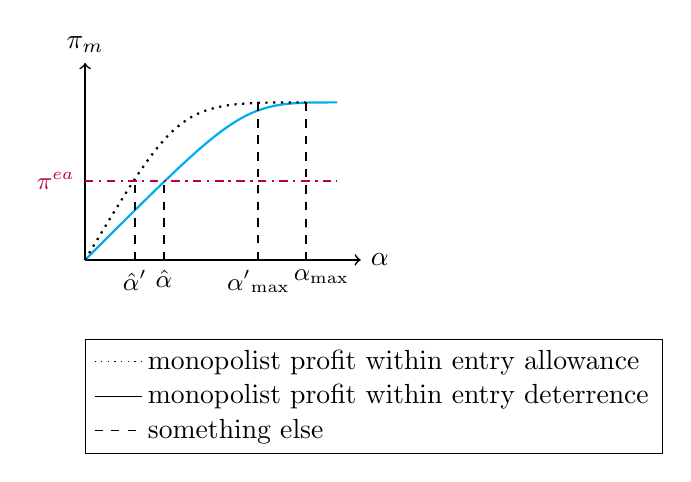
\begin{tikzpicture}
   \draw[semithick,->] (0,0) -- (3.5,0) node[right] {$ \alpha $};
   \draw[semithick,->] (0,0) -- (0,2.5) node[above]  {$ \pi_m $};  
 
   \path[thick,cyan,draw]     (0,0) node[right]{} .. controls (2,2) .. (3.2,2);
   \path[thick,dotted,draw]   (0,0) node[right]{} .. controls (1.2,2) .. (2.8,2);
   \path[thick,dashed,draw]   (2.2,0) node[below]{\small $\alpha{'}_{\max}$} .. controls (2.2,0) .. (2.2,2);
   \path[thick,dashed,draw]   (0.631,0) node[below]{\small $\hat{ \alpha}{'}$} .. controls (0.631,1) .. (0.631,1);
 
   \path[thick,dashdotted,draw,purple]   (0,1) node[left]{\small $\pi^{ea}$}
     .. controls (2,1) ..     (3.2,1);
   \path[thick,dashed,draw]   (2.8,2) node[above]{}
     .. controls (2.8,0) ..   (2.8,0);
   \path[thick,dashed,draw]   (3,0) node[below]{\small $\alpha_{\max}$}
         .. controls (3,0) .. (3,0);
   \path[thick,dashed,draw]   (1,0) node[below]{\small $\hat{\alpha}$}
         .. controls (1,1) .. (1,1);
 
   \begin{tikzlegend}[legend entries={monopolist profit within entry allowance,
      monopolist profit within entry deterrence,something else},
        legend style={at={(0,-1)},anchor=north west}, legend cell align=left]
     \addlegendimage{dotted,sharp plot}
     \addlegendimage{sharp plot}
     \addlegendimage{dashed, sharp plot}
   \end{tikzlegend}
\end{tikzpicture}

\clearpage
\newpage
\section{Flowchart}
\begin{center}
	% ---------------- flowchart ---------------

\centering
\begin{tikzpicture}[
	io/.style={trapezium, trapezium left angle=70, trapezium right angle=110, fill=magenta!10, draw=magenta},
    op/.style={rectangle, fill=orange!10, draw=orange},
    cn/.style={diamond, aspect=2, inner sep=2pt, fill=red!10, draw=red},
    node distance=5mm, thick]
    \node[io] (in) {Input $a,b$};
    \node[op, below=of in] (div) {$r=a \mod b$};
    \node[op, below=of div] (set) {$a=b,\ b=r$};
    \node[cn, below=of set] (cond) {$b=0?$};
    \node[io, below=of cond] (out) {Output $a$};
    %
    \path[->]
      (in) edge (div)
      (div) edge (set)
      (set) edge (cond)
      (cond) edge node[right] {Yes} (out);
    \draw[->] (cond) -- node[below] {No} ++(1.5,0) |- (div);

\end{tikzpicture}
\break
%%--------------------------------------
\end{center}

%----------------------------------
\section{Nodes}
\begin{center}
	This is the node tree for searching algorithm. Different colors indicate different level of searching steps. %\vskip 0.5cm


\tikzset{
	level/.style={sibling distance=35mm/#1},
	treenode/.style={align=center,inner sep=0pt},
	% Black nodes
	node_black/.style={treenode,circle,black,draw=black,very thick,text width=0.5cm},
	% Red nodes
	node_red/.style={treenode,circle,red,draw=red,very thick,text width=0.5cm},
	% Blue nodes
	node_blue/.style={treenode,circle,blue,draw=blue,very thick,text width=0.5cm},
	% Nil nodes
	node_nil/.style={treenode,rectangle,fill=black,minimum width=0.3cm,minimum height=0.3cm}
}
\begin{tikzpicture}
\node[node_red] (z){$S$}
  child {node[node_black] (a) {$R$}								%%% Right
    child[black] {node[node_black]  (b) {$R$}
      child {node (b1) {$\vdots$}
       child {node[node_black] (b11) {$R$}}
      }
      child {node (b2) {$\vdots$}
       child {node[node_black] (b12) {$U$}}
      }
    }
    child[black] {node[node_black] (g) {$D$}
      child {node (g1) {$\vdots$}
       child {node[node_black] (g11) {$R$}}
      }
      child {node (g2) {$\vdots$}
       child {node[node_black] (g12) {$U$}}
      }
    }
  }
   child[red] {node[node_red] (d) {$L$}                    %%%% LEft - the shortest parth
      child[black] {node[node_black]  (e) {$L$}
        child {node (e1) {$\vdots$}
         child {node[node_black] (e11) {$R$}}
        }
        child {node (e2) {$\vdots$}
         child {node[node_black] (e12) {$L$}}
        }
      }
      child[red] {node[node_red] (f) {$D$}
        child[black] {node (f1) {$\vdots$}
         child[black] {node[node_black] (f11) {$U$}}
        }
        child[red] {node (f2) {$\vdots$}
         child[red] {node[node_red] (f12) {$D$}}
        }
      }
    }
    child[black] {node[node_black] (m) {$U$}      %%% Up
      child {node[node_black]  (n) {$U$}
        child {node (n1) {$\vdots$}
         child {node[node_black] (n11) {$R$}}
        }
        child {node (n2) {$\vdots$}
         child {node[node_black] (n12) {$L$}}
        }
      }
      child {node[node_black] (o) {$L$}
        child {node (o1) {$\vdots$}
         child {node[node_black] (o11) {$U$}}
        }
        child {node (o2) {$\vdots$}
         child[blue] {node[node_blue] (o12) {$R$}}
        }
      }
    }
  child[black] {node[node_black]  (j) {$D$}   %%% Down
    child {node[node_black] (k) {$D$}
      child {node {$\vdots$}
       child[blue] {node[node_blue] (k11) {$R$}}
      }
      child {node {$\vdots$}
       child {node[node_black] (k12) {$D$}}
      }
    }
    child {node[node_black] (l) {$L$}
    child {node {$\vdots$}
     child {node[node_black] (l11) {$U$}}
    }
    child {node (c){$\vdots$}
     child {node[node_black] (l12) {$L$}
            child [grow=right] {node (r) {$level^n$} edge from parent[draw=none]
              child [grow=up] {node (s) {$\vdots$} edge from parent[draw=none]
                child [grow=up] {node (t) {$level^2$} edge from parent[draw=none]
                  child [grow=up] {node (u) {$level^1$} edge from parent[draw=none]
                   child [grow=up] {node (u) {$root$} edge from parent[draw=none]}
                                   }
                                 }
                               }
                               }
            }
          }
         }
};
\path (b) -- (g) node [midway] {$\cdots$};\path (n) -- (o) node [midway] {$\cdots$};
\path (e) -- (f) node [midway] {$\cdots$};
\path (k) -- (l) node [midway] {$\cdots$};
\path (b11) -- (b12) node [midway] {$\cdots$};
\path (g11) -- (g12) node [midway] {$\cdots$};\path (n11) -- (n12) node [midway] {$\cdots$};
\path (e11) -- (e12) node [midway] {$\cdots$};\path (o11) -- (o12) node [midway] {$\cdots$};
\path (f11) -- (f12) node [midway] {$\cdots$};
\path (k11) -- (k12) node [midway] {$\cdots$};
\path (l11) -- (l12) node [midway] {$\cdots$};
\end{tikzpicture}

%% take notes


\begin{tikzpicture}
%\node[node_black] (n12) {}
%\node[node_red] (n12) {}
%\node[node_blue] (n12) {}
\end{tikzpicture}


\end{center}

%----------------------------------
\newpage
\section{Grap-Automata}
\begin{figure}[h!]
	\begin{center}
		%--- using \usetikzlibrary{automata}
%\newpage
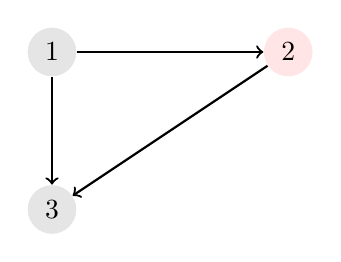
\begin{tikzpicture}
	\tikzstyle{vertex}=[circle,fill=black!10]
	\tikzstyle{selected vertex}=[vertex,fill=red!10]
	\tikzstyle{edge}=[->,thick]
	
	\node[vertex](v1) at (0,0){1};
	\node[selected vertex](v2) at (3,0){2};
	\node[vertex](v3) at (0,-2){3};	
	
	\draw[edge](v1)--(v2);
	\draw[edge](v1)--(v3);
	\draw[edge](v2)--(v3);	
\end{tikzpicture}
\caption{Example1}

\vspace{30pt}

\begin{tikzpicture}[->,node distance=3cm,auto]
	\node[initial,state](A){$q_1$};
	\node[state](B)[right of=A]{$q_2$};
	\node[state](C)[right of=B]{$q_3$};
	\node[state,accepting](D)[below of=B]{$q_4$};
	
	\path(A)edge[loop above]node{$1\rightarrow H,L$}(A)
			edge [bend left] node{$H \rightarrow 1,R$}(B)
		 (B)edge[loop above]node{b}(B)
		    edge [bend left] node{$H \rightarrow 1,L$}(A)
			edge node{$x_1$}(C)
    	 (C)edge[loop above]node{b}(C)
    	    edge node{$x_2$}(D)
	;	
\end{tikzpicture}
\caption{Example2}

\vspace{30pt}

\begin{tikzpicture}[->,node distance=3cm,auto]
	\node[initial,state](A){$A$};
	\node[state](B)[right of=A]{$B$};
	\node[state](C)[below of=A]{$C$};
	\node[state](D)[below of=B]{$D$};
	\node[state](E)[right of=D]{$E$};
	
	\path(A)edge[bend left](B)
	        edge(B)		 
		 (B)edge[bend left](A)
			edge(D)
    	 (C)edge(A)
    	    edge[loop below](C)
    	 (D)edge(C)
    	    edge(E)  
	;	
\end{tikzpicture}
\caption{This is node graph}
	\end{center}
\end{figure}

%----------------------------------
\newpage
\section{Plotting Data}
\begin{figure}[ht]
	\begin{center}
		%\newpage
\begin{tikzpicture}
    \begin{axis}[name=plot, xlabel={x(Ns/m)},ylabel={y(J)},ymin=0,ymax=1.6]
    
    \addplot[black,mark=triangle*] table{./data/friction.txt};\label{f}
    \addplot[red,mark=o] table{./data/generator.txt};\label{g}
    \addplot[blue] table{./data/simulated_total.txt};\label{s}
    \addplot[green,dashed] table{./data/theoretical_total.txt};\label{t}
	
	% Define two points for drawing an arrow to the "matched" point
%    \node[] (C) at (axis cs: 1,0.5) {};
%    \node[] (B) at (axis cs: 2.5,0.5) {};
    \end{axis}
	
	% Create a node to act as the legend  
    \node[anchor=north,fill=white,draw=black] (legend) at 
    ($(plot.north east)-(0 mm, 1 mm)$){
    	\begin{tabular}{l l}
        	f & \ref{f} \\
	        g & \ref{g} \\
    	    s & \ref{s} \\
        	t & \ref{t} \\
	    \end{tabular} 
	    };
    
%	\draw[triangle 45-] (C.east)--(B.west);
%	\node[anchor=west] (label) at (B) {matched};

\end{tikzpicture}
\caption{Example of plotting data1}

\vspace{30pt}

\begin{tikzpicture}
    \begin{axis}[name=plot, xlabel={x(Ns/m)},ylabel={y(J)},ymin=0,ymax=1.6]
    
    \addplot[black,mark=triangle*] table{./data/friction.txt};\label{f}
    \addplot[red,mark=o] table{./data/generator.txt};\label{g}
    \addplot[blue] table{./data/simulated_total.txt};\label{s}
    \addplot[green,dashed] table{./data/theoretical_total.txt};\label{t}
	
	% Define two points for drawing an arrow to the "matched" point
    \node[] (C) at (axis cs: 1,.5) {};
    \node[] (B) at (axis cs: 2.5,.5) {};
    \end{axis}
	
	% Create a node to act as the legend  
    \node[anchor=north,fill=white,draw=black] (legend) at ($(plot.north)-(0 mm, 1 mm)$) {\begin{tabular}{l l l l}
        f & \ref{f}  & g & \ref{g} \\
        s & \ref{s}  & t & \ref{t} \\
    \end{tabular} };
    
	\draw[triangle 45-] (C.east)--(B.west);
	\node[anchor=west] (label) at (B) {matched};

\end{tikzpicture}
\caption{Example of plotting data2}

\vspace{30pt}
	\end{center}
\end{figure}

%----------------------------------
\newpage
\section{Rotation Geometry}
\begin{figure}[ht]
	\begin{center}
		%---
%
%
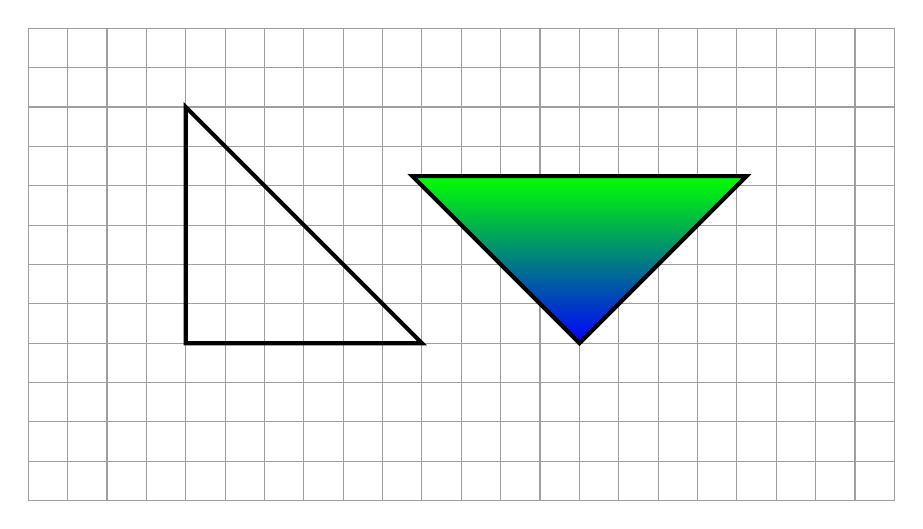
\begin{tikzpicture}
	\draw[step=0.5,gray!75](-2,-2) grid(9,4); %from (-2,-2) to (9,4)
	\draw[line width=1.5pt](0,0)--(3,0)--(0,3)--cycle;
	\draw[line width=1.5pt, xshift=5cm, rotate=45, bottom color = blue, top color=green](0,0)--(3,0)--(0,3)--cycle;
\end{tikzpicture}
\caption{Rotation Triangular}


	\end{center}
\end{figure} 

%--------- draw SimplePolygon.tex-------
\section{Draw Simple Polygon}
\begin{figure}[ht]
	\begin{center}
		
\begin{tikzpicture}[scale=1.5, transform shape]
	
			\tkzInit[xmin=-3,xmax=4.5, ymin=-.5, ymax=2.8]
			\tkzClip
			
			\tkzDefPoint(0,0){A}
			\tkzDefPoint(4,0){B}
			\tkzDefPoint(130:3){C}
			
			
			
			\tkzDefLine[orthogonal=through C](A,B)\tkzGetPoint{c}
			\tkzInterLL(A,B)(C,c)\tkzGetPoint{C'}
			
	
			\tkzMarkAngle[size=.5,arrows=->,>=stealth,color=red](B,A,C)
			\tkzMarkAngle[size=.4,arrows=->,>=stealth,color=blue](C,A,C')
			\tkzMarkRightAngle[size=.3,fill=blue!20,draw opacity=0](A,C',C)
			
			
			\tkzDrawSegment[dashed](C,C')
			\tkzDrawLine[add=0cm and 1cm,dashed](A,C')
			
			
			
			\tkzDrawPolygon(A,B,C)
			\tkzDrawPoints(A,B,C,C')
			\tkzLabelPoints[below](A,C')
			\tkzLabelPoints[right](B)
			\tkzLabelPoints[above](C)
			
			\begin{scope}[font=\footnotesize]
			\tkzLabelSegment[below](A,B){$c$}
			\tkzLabelSegment(A,C){$b$}
			\tkzLabelSegment[above](B,C){$a$}
			\tkzLabelSegment[left](C,C'){$h$}
			\tkzLabelAngle[pos=.7](B,A,C){$\widehat{A}$}
			\tkzLabelAngle[pos=1.1,below](C,A,C'){$\ang{180}-\widehat{A}$}
			\end{scope}
			
\end{tikzpicture}
\caption{Draw Polygon with  }
	\end{center}
\end{figure} 

%--Parallelepiped.tex--
\section{Draw Rectangle Polygon}
\begin{figure}[ht]
	\begin{center}
		%
% link http://www.texample.net/tikz/examples/parallelepiped/
%
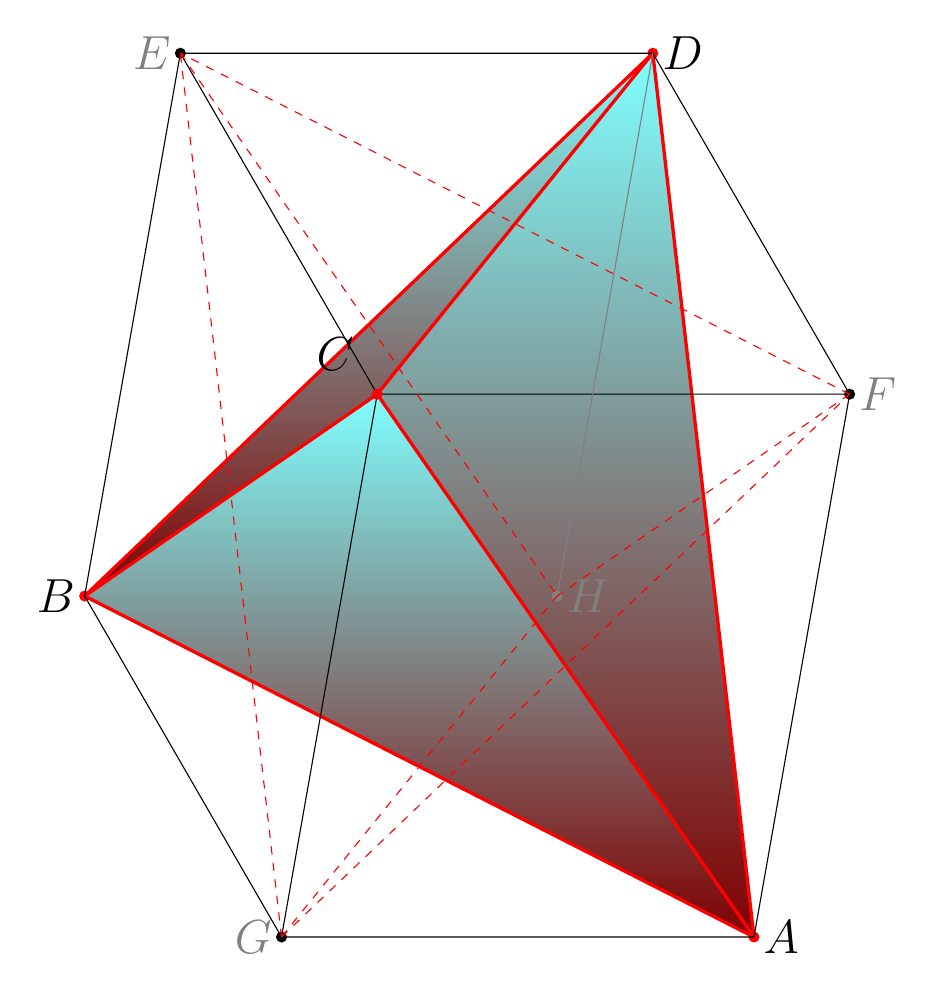
\begin{tikzpicture}[font=\LARGE] 

% Figure parameters (tta and k needs to have the same sign)
% They can be modified at will
\def \tta{ -10.00000000000000 } % Defines the first angle of perspective
\def \k{    -3.00000000000000 } % Factor for second angle of perspective
\def \l{     6.00000000000000 } % Defines the width  of the parallelepiped
\def \d{     5.00000000000000 } % Defines the depth  of the parallelepiped
\def \h{     7.00000000000000 } % Defines the heigth of the parallelepiped

% The vertices A,B,C,D define the reference plan (vertical)
\coordinate (A) at (0,0); 
\coordinate (B) at ({-\h*sin(\tta)},{\h*cos(\tta)}); 
\coordinate (C) at ({-\h*sin(\tta)-\d*sin(\k*\tta)},
                    {\h*cos(\tta)+\d*cos(\k*\tta)}); 
\coordinate (D) at ({-\d*sin(\k*\tta)},{\d*cos(\k*\tta)}); 

% The vertices Ap,Bp,Cp,Dp define a plane translated from the 
% reference plane by the width of the parallelepiped
\coordinate (Ap) at (\l,0); 
\coordinate (Bp) at ({\l-\h*sin(\tta)},{\h*cos(\tta)}); 
\coordinate (Cp) at ({\l-\h*sin(\tta)-\d*sin(\k*\tta)},
                     {\h*cos(\tta)+\d*cos(\k*\tta)}); 
\coordinate (Dp) at ({\l-\d*sin(\k*\tta)},{\d*cos(\k*\tta)}); 

% Marking the vertices of the tetrahedron (red)
% and of the parallelepiped (black)
\fill[black]  (A) circle [radius=2pt]; 
\fill[red]    (B) circle [radius=2pt]; 
\fill[black]  (C) circle [radius=2pt]; 
\fill[red]    (D) circle [radius=2pt]; 
\fill[red]   (Ap) circle [radius=2pt]; 
\fill[black] (Bp) circle [radius=2pt]; 
\fill[red]   (Cp) circle [radius=2pt]; 
\fill[black] (Dp) circle [radius=2pt]; 

% painting first the three visible faces of the tetrahedron
\filldraw[draw=red,bottom color=red!50!black, top color=cyan!50]
  (B) -- (Cp) -- (D);
\filldraw[draw=red,bottom color=red!50!black, top color=cyan!50]
  (B) -- (D)  -- (Ap);
\filldraw[draw=red,bottom color=red!50!black, top color=cyan!50]
  (B) -- (Cp) -- (Ap);

% Draw the edges of the tetrahedron
\draw[red,-,very thick] (Ap) --  (D)
                        (Ap) --  (B)
                        (Ap) -- (Cp)
                        (B)  --  (D)
                        (Cp) --  (D)
                        (B)  -- (Cp);

% Draw the visible edges of the parallelepiped
\draw [-,thin] (B)  --  (A)
               (Ap) -- (Bp)
               (B)  --  (C)
               (D)  --  (C)
               (A)  --  (D)
               (Ap) --  (A)
               (Cp) --  (C)
               (Bp) --  (B)
               (Bp) -- (Cp);

% Draw the hidden edges of the parallelepiped
\draw [gray,-,thin] (Dp) -- (Cp);
                    (Dp) --  (D);
                    (Ap) -- (Dp);

% Name the vertices (the names are not consistent
%  with the node name, but it makes the programming easier)
\draw (Ap) node [right]           {$A$}
      (Bp) node [right, gray]     {$F$}
      (Cp) node [right]           {$D$}
      (C)  node [left,gray]       {$E$}
      (D)  node [left]            {$B$}
      (A)  node [left,gray]       {$G$}
      (B)  node [above left=+5pt] {$C$}
      (Dp) node [right,gray]      {$H$};

% Drawing again vertex $C$, node (B) because it disappeared behind the edges.
% Drawing again vertex $H$, node (Dp) because it disappeared behind the edges.
\fill[red]   (B) circle [radius=2pt]; 
\fill[gray] (Dp) circle [radius=2pt]; 

% From the reference and this example one can easily draw 
% the twin tetrahedron jointly to this one.
% Drawing the edges of the twin tetrahedron
% switching the p_s: A <-> Ap, etc...
\draw[red,-,dashed, thin] (A)  -- (Dp)
                          (A)  -- (Bp)
                          (A)  --  (C)
                          (Bp) -- (Dp)
                          (C)  -- (Dp)
                          (Bp) --  (C);
                          
\end{tikzpicture}
	\end{center}
\end{figure}
\newpage
\section{Draw Sphere}
%%%%%%%%%%%%%%%%%%%%%%%%%%%%%%%%%%%%%%%%%%%%%%%%%%%%%%%%%%%%%%%
%
% Welcome to Overleaf --- just edit your LaTeX on the left,
% and we'll compile it for you on the right. If you open the
% 'Share' menu, you can invite other users to edit at the same
% time. See www.overleaf.com/learn for more info. Enjoy!
%
%%%%%%%%%%%%%%%%%%%%%%%%%%%%%%%%%%%%%%%%%%%%%%%%%%%%%%%%%%%%%%%
% Stereographic and cylindrical map projections
% Author: Tomasz M. Trzeciak
% Source: LaTeX-Community.org 
%         <http://www.latex-community.org/viewtopic.php?f=4&t=2111>
%%%%%%%%%%%%%%%%%%%%%%%%%%%%%%%%%%%%%%%%%%%%%%%%%%%%%%%%%%%%%%%



%\documentclass{article}
%\usepackage{tikz}
\usetikzlibrary{calc,fadings,decorations.pathreplacing}
%\usepackage{verbatim}

%\usepackage{biblatex}

\begin{comment}

:Title: Stereographic and cylindrical map projections
:Tags: 3D
:Slug: map-projections
:Grid: 2x2

Examples inspired by the thread at comp.text.tex about `how to convert some hand
drawn pictures into programmatic 3D sketches`__.

.. __: http://groups.google.com/group/comp.text.tex/browse_thread/thread/a03baf5d6fa64865/f7e7b903f1d87a6a

The sketches present stereographic and cylindrical map projections and they
pose some interesting challenges for doing them with a 2D drawing package PGF/TikZ.

The main idea is to draw in selected 3D planes and then project onto the canvas
coordinate system with an appriopriate transformation. Some highlights:

- usage of pgf math engine for calculation of projection transformations and
  transitions points from visible (solid lines) to invisible (dashed lines) on
  meridians and latitude circles
- definition of 3D plane transformation with expanded styles so that they are robust
  against redefinition of macros used in their construction
- usage of named coordinates (nodes) for definition of characteristic points in
  local coordinate systems so that they are accessible outside of their plane of
  definition
- calculation of intersections points with TikZ intersection coordinate system
- usage of 'to' path operation instead of 'arc' for marking angles to allow for
  easy positioning of text labels on the curve
- 3D lighting effects with shading

:Author: Tomasz M. Trzeciak
:Source: LaTeX-Community.org_

.. _LaTeX-Community.org: http://www.latex-community.org/viewtopic.php?f=4&t=2111

\end{comment}

%% helper macros

\newcommand\pgfmathsinandcos[3]{%
  \pgfmathsetmacro#1{sin(#3)}%
  \pgfmathsetmacro#2{cos(#3)}%
}
\newcommand\LongitudePlane[3][current plane]{%
  \pgfmathsinandcos\sinEl\cosEl{#2} % elevation
  \pgfmathsinandcos\sint\cost{#3} % azimuth
  \tikzset{#1/.style={cm={\cost,\sint*\sinEl,0,\cosEl,(0,0)}}}
}
\newcommand\LatitudePlane[3][current plane]{%
  \pgfmathsinandcos\sinEl\cosEl{#2} % elevation
  \pgfmathsinandcos\sint\cost{#3} % latitude
  \pgfmathsetmacro\yshift{\cosEl*\sint}
  \tikzset{#1/.style={cm={\cost,0,0,\cost*\sinEl,(0,\yshift)}}} %
}
\newcommand\DrawLongitudeCircle[2][1]{
  \LongitudePlane{\angEl}{#2}
  \tikzset{current plane/.prefix style={scale=#1}}
   % angle of "visibility"
  \pgfmathsetmacro\angVis{atan(sin(#2)*cos(\angEl)/sin(\angEl))} %
  \draw[current plane] (\angVis:1) arc (\angVis:\angVis+180:1);
  \draw[current plane,dashed] (\angVis-180:1) arc (\angVis-180:\angVis:1);
}
\newcommand\DrawLatitudeCircle[2][1]{
  \LatitudePlane{\angEl}{#2}
  \tikzset{current plane/.prefix style={scale=#1}}
  \pgfmathsetmacro\sinVis{sin(#2)/cos(#2)*sin(\angEl)/cos(\angEl)}
  % angle of "visibility"
  \pgfmathsetmacro\angVis{asin(min(1,max(\sinVis,-1)))}
  \draw[current plane] (\angVis:1) arc (\angVis:-\angVis-180:1);
  \draw[current plane,dashed] (180-\angVis:1) arc (180-\angVis:\angVis:1);
}

%% document-wide tikz options and styles

\tikzset{%
  >=latex, % option for nice arrows
  inner sep=0pt,%
  outer sep=2pt,%
  mark coordinate/.style={inner sep=0pt,outer sep=0pt,minimum size=3pt,
    fill=black,circle}%
}

%\begin{document}

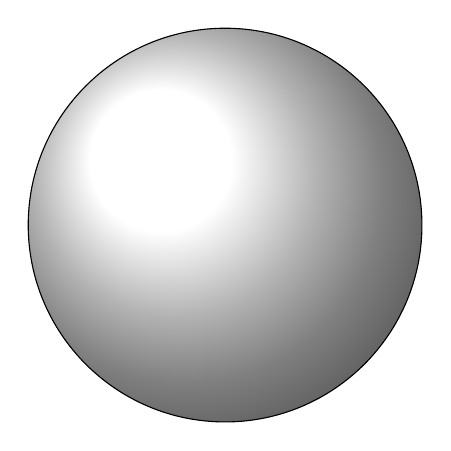
\begin{tikzpicture} % "THE GLOBE" showcase

\def\R{2.5} % sphere radius
\def\angEl{35} % elevation angle
\filldraw[ball color=white] (0,0) circle (\R);
\foreach \t in {-80,-60,...,80} { \DrawLatitudeCircle[\R]{\t} }
\foreach \t in {-5,-35,...,-175} { \DrawLongitudeCircle[\R]{\t} }

\end{tikzpicture}

\begin{tikzpicture} % CENT

%% some definitions

\def\R{2.5} % sphere radius
\def\angEl{35} % elevation angle
\def\angAz{-105} % azimuth angle
\def\angPhi{-40} % longitude of point P
\def\angBeta{19} % latitude of point P

%% working planes

\pgfmathsetmacro\H{\R*cos(\angEl)} % distance to north pole
\tikzset{xyplane/.style={cm={cos(\angAz),sin(\angAz)*sin(\angEl),-sin(\angAz),
                              cos(\angAz)*sin(\angEl),(0,-\H)}}}
\LongitudePlane[xzplane]{\angEl}{\angAz}
\LongitudePlane[pzplane]{\angEl}{\angPhi}
\LatitudePlane[equator]{\angEl}{0}

%% draw xyplane and sphere

\draw[xyplane] (-2*\R,-2*\R) rectangle (2.2*\R,2.8*\R);
\fill[ball color=white] (0,0) circle (\R); % 3D lighting effect
\draw (0,0) circle (\R);

%% characteristic points

\coordinate (O) at (0,0);
\coordinate[mark coordinate] (N) at (0,\H);
\coordinate[mark coordinate] (S) at (0,-\H);
\path[pzplane] (\angBeta:\R) coordinate[mark coordinate] (P);
\path[pzplane] (\R,0) coordinate (PE);
\path[xzplane] (\R,0) coordinate (XE);
\path (PE) ++(0,-\H) coordinate (Paux); % to aid Phat calculation
\coordinate[mark coordinate] (Phat) at (intersection cs: first line={(N)--(P)},
                                        second line={(S)--(Paux)});

%% draw meridians and latitude circles

\DrawLatitudeCircle[\R]{0} % equator
%\DrawLatitudeCircle[\R]{\angBeta}
\DrawLongitudeCircle[\R]{\angAz} % xzplane
\DrawLongitudeCircle[\R]{\angAz+90} % yzplane
\DrawLongitudeCircle[\R]{\angPhi} % pzplane

%% draw xyz coordinate system

\draw[xyplane,<->] (1.8*\R,0) node[below] {$x,\xi$} -- (0,0) -- (0,2.4*\R)
    node[right] {$y,\eta$};
\draw[->] (0,-\H) -- (0,1.6*\R) node[above] {$z,\zeta$};

%% draw lines and put labels

\draw[dashed] (P) -- (N) +(0.3ex,0.6ex) node[above left] {$\mathbf{N}$};
\draw (P) -- (Phat) node[above right] {$\mathbf{\hat{P}}$};
\path (S) +(0.4ex,-0.4ex) node[below] {$\mathbf{S}$};
\draw[->] (O) -- (P) node[above right] {$\mathbf{P}$};
\draw[dashed] (XE) -- (O) -- (PE);
\draw[pzplane,->,thin] (0:0.5*\R) to[bend right=15]
    node[pos=0.4,right] {$\beta$} (\angBeta:0.5*\R);
\draw[equator,->,thin] (\angAz:0.4*\R) to[bend right=30]
    node[pos=0.4,below] {$\phi$} (\angPhi:0.4*\R);
\draw[thin,decorate,decoration={brace,raise=0.5pt,amplitude=1ex}] (N) -- (O)
    node[midway,right=1ex] {$a$};

\end{tikzpicture}

\begin{tikzpicture} % MERC

%% some definitions

\def\R{3} % sphere radius
\def\angEl{25} % elevation angle
\def\angAz{-100} % azimuth angle
\def\angPhiOne{-50} % longitude of point P
\def\angPhiTwo{-35} % longitude of point Q
\def\angBeta{33} % latitude of point P and Q

%% working planes

\pgfmathsetmacro\H{\R*cos(\angEl)} % distance to north pole
\LongitudePlane[xzplane]{\angEl}{\angAz}
\LongitudePlane[pzplane]{\angEl}{\angPhiOne}
\LongitudePlane[qzplane]{\angEl}{\angPhiTwo}
\LatitudePlane[equator]{\angEl}{0}

%% draw background sphere

\fill[ball color=white] (0,0) circle (\R); % 3D lighting effect
%\fill[white] (0,0) circle (\R); % just a white circle
\draw (0,0) circle (\R);

%% characteristic points

\coordinate (O) at (0,0);
\coordinate[mark coordinate] (N) at (0,\H);
\coordinate[mark coordinate] (S) at (0,-\H);
\path[xzplane] (\R,0) coordinate (XE);
\path[pzplane] (\angBeta:\R) coordinate (P);
\path[pzplane] (\R,0) coordinate (PE);
\path[qzplane] (\angBeta:\R) coordinate (Q);
\path[qzplane] (\R,0) coordinate (QE);

%% meridians and latitude circles

% \DrawLongitudeCircle[\R]{\angAz} % xzplane
% \DrawLongitudeCircle[\R]{\angAz+90} % yzplane
\DrawLongitudeCircle[\R]{\angPhiOne} % pzplane
\DrawLongitudeCircle[\R]{\angPhiTwo} % qzplane
\DrawLatitudeCircle[\R]{\angBeta}
\DrawLatitudeCircle[\R]{0} % equator

% shifted equator in node with nested call to tikz 
% (I didn't know it's possible)
\node at (0,1.6*\R) { \tikz{\DrawLatitudeCircle[\R]{0}} };

%% draw lines and put labels

\draw (-\R,-\H) -- (-\R,2*\R) (\R,-\H) -- (\R,2*\R);
\draw[->] (XE) -- +(0,2*\R) node[above] {$y$};
\node[above=8pt] at (N) {$\mathbf{N}$};
\node[below=8pt] at (S) {$\mathbf{S}$};
\draw[->] (O) -- (P);
\draw[dashed] (XE) -- (O) -- (PE);
\draw[dashed] (O) -- (QE);
\draw[pzplane,->,thin] (0:0.5*\R) to[bend right=15]
    node[midway,right] {$\beta$} (\angBeta:0.5*\R);
\path[pzplane] (0.5*\angBeta:\R) node[right] {$\hat{1}$};
\path[qzplane] (0.5*\angBeta:\R) node[right] {$\hat{2}$};
\draw[equator,->,thin] (\angAz:0.5*\R) to[bend right=30]
    node[pos=0.4,above] {$\phi_1$} (\angPhiOne:0.5*\R);
\draw[equator,->,thin] (\angAz:0.6*\R) to[bend right=35]
    node[midway,below] {$\phi_2$} (\angPhiTwo:0.6*\R);
\draw[equator,->] (-90:\R) arc (-90:-70:\R) node[below=0.3ex] {$x = a\phi$};
\path[xzplane] (0:\R) node[below] {$\beta=0$};
\path[xzplane] (\angBeta:\R) node[below left] {$\beta=\beta_0$};

\end{tikzpicture}


\begin{tikzpicture} % KART

\def\R{2.5}

\node[draw,minimum size=2cm*\R,inner sep=0,outer sep=0,circle] (C) at (0,0) {};
\coordinate (O) at (0,0);
\coordinate[mark coordinate] (Phat) at (20:2.5*\R);
\coordinate (T1) at (tangent cs: node=C, point={(Phat)}, solution=1);
\coordinate (T2) at (tangent cs: node=C, point={(Phat)}, solution=2);
\coordinate[mark coordinate] (P) at ($(T1)!0.5!(T2)$);

\draw[dashed] (T1) -- (O) -- (T2) -- (Phat) -- (T1) -- (T2);
\draw[<->] (0,1.5*\R) node[above] {$y$} |- (2.5*\R,0) node[right] {$x$};
\draw (O) node[below left] {$\mathbf{O}$} -- (P)
    +(1ex,0) node[above=1ex] {$\mathbf{P}$};
\draw (P) -- (Phat) node[above=1ex] {$\mathbf{\hat{P}}$};

\end{tikzpicture}

%\printbibliography
%\end{document}



\printbibliography
\end{document}